%%%%%%%%%%%%%%%%%%%%%%%%%%%%%%%%%%%%%%%%%%%%%%%%%%%%%%%%%%%%%%%
%%%%% CHOOSE PAGE LAYOUT
\documentclass[a4paper,twoside]{ociamthesis}
% This one will format for one-sided binding (ie left margin > right margin; no extra blank pages):
%\documentclass[a4paper]{ociamthesis}
% This one will format for PDF output (ie equal margins, no extra blank pages):
%\documentclass[a4paper,nobind]{ociamthesis} 



%%%%% SELECT YOUR DRAFT OPTIONS
%\fancyfoot[C]{\emph{DRAFT Printed on \today}}  
\correctionstrue


%%%%% BIBLIOGRAPHY SETUP
% The science-type option: numerical in-text citation with references in order of appearance.
\usepackage[style=numeric-comp, sorting=none, backend=biber, doi=false, isbn=false]{biblatex}
\newcommand*{\bibtitle}{References}

% This makes the bibliography left-aligned (not 'justified') and slightly smaller font.
\renewcommand*{\bibfont}{\raggedright\small}
\addbibresource{references.bib}


%%%%% THESIS / TITLE PAGE INFORMATION
% Everybody needs to complete the following:
\title{Towards Design and Control \\ of Soft Robots}
\author{Brandon Jonathan Caasenbrood}
\college{Department of Mechanical Engineering}
\degree{Doctor of Philosophy}
\degreedate{May 2022}


\AtBeginDocument{\colorlet{chaptergrey}{pyblue!50}}


%%%%% THE ACTUAL DOCUMENT STARTS HERE
\begin{document}

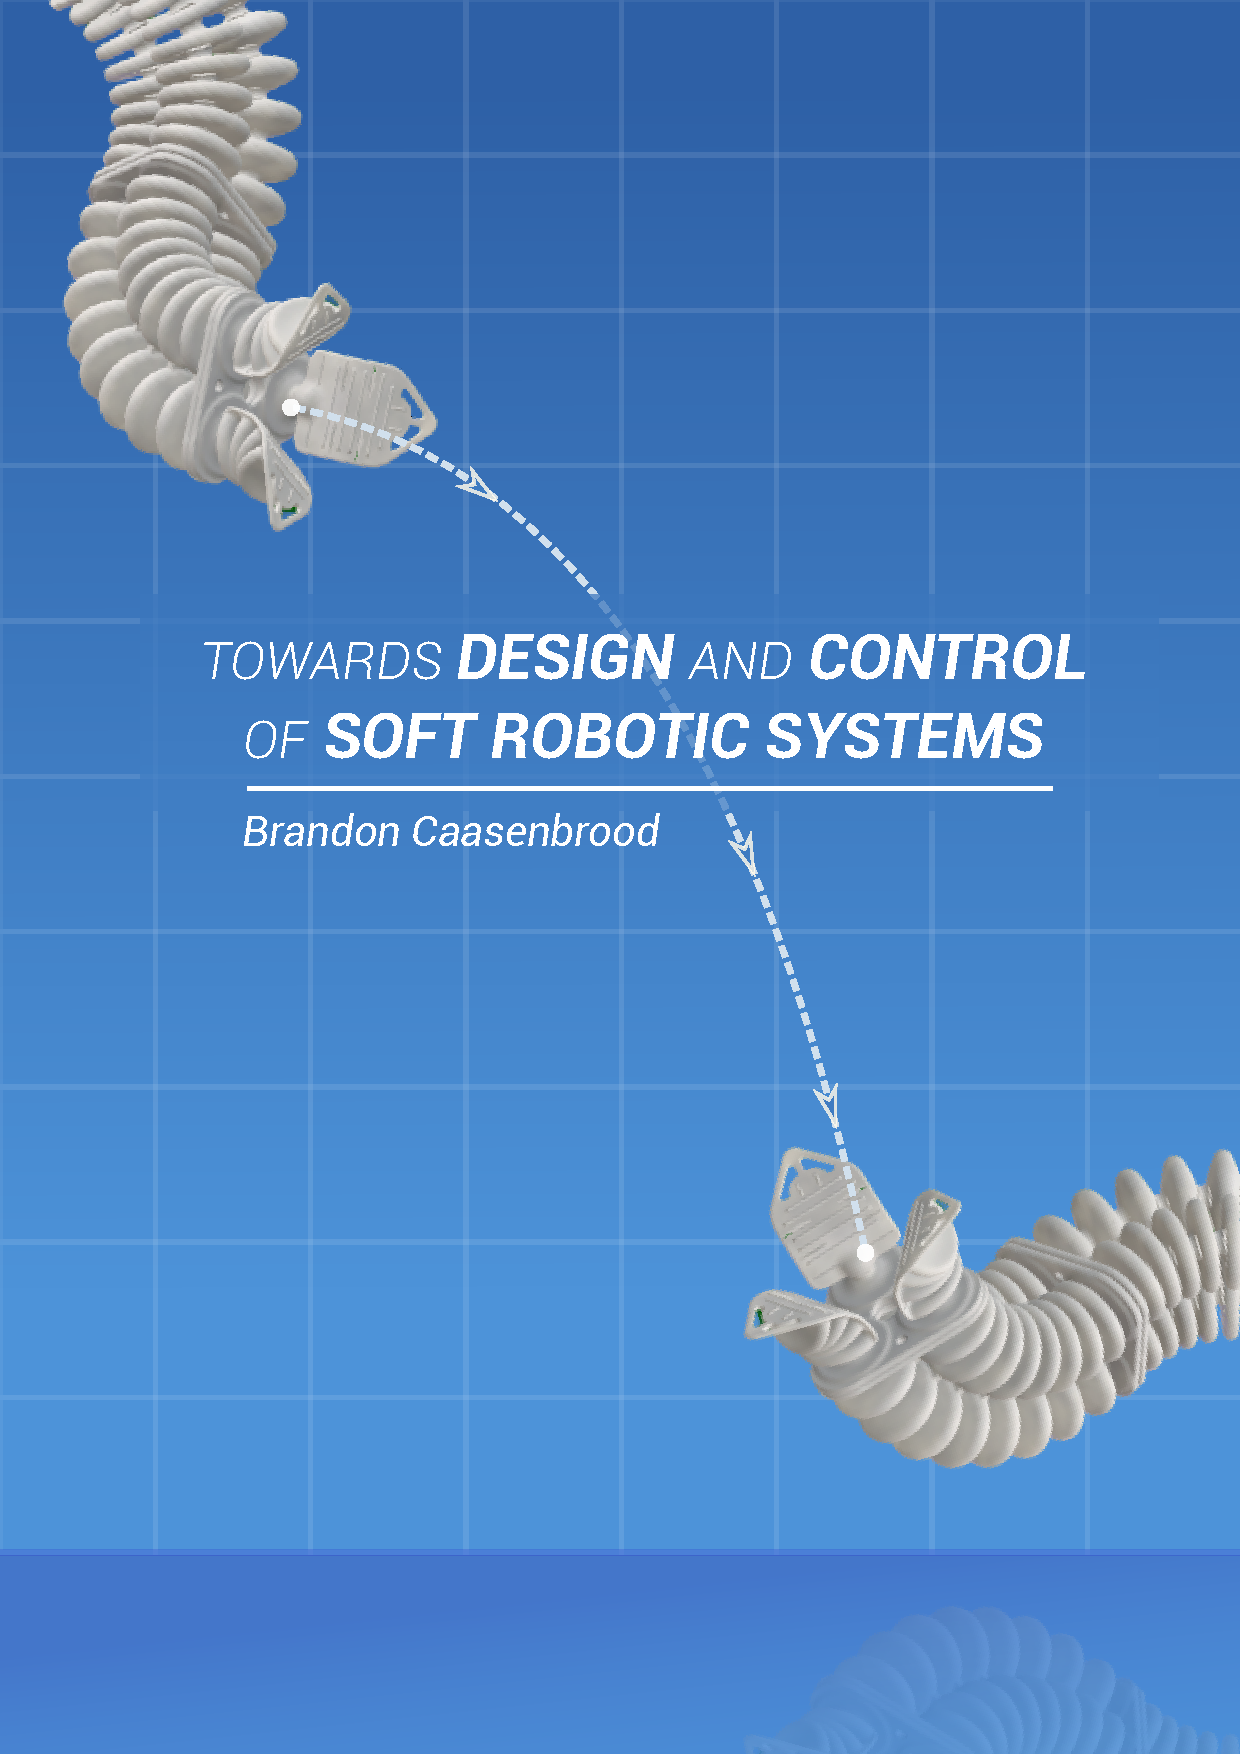
\includepdf[page=1]{./cover/cover-1.pdf}
%\maketitle
%%%%% CHOOSE YOUR LINE SPACING HERE
% This is the official option.  Use it for your submission copy and library copy:
%\setlength{\textbaselineskip}{22pt plus2pt}
% This is closer spacing (about 1.5-spaced) that you might prefer for your personal copies:
%\setlength{\textbaselineskip}{19pt plus1pt minus1pt}
\setlength{\baselineskip}{\frontmatterbaselineskip}
%\setlength{\textbaselineskip}{16pt plus2pt minus1pt}
%\setlength{\frontmatterbaselineskip}{17pt plus1pt minus1pt}
%\setlength{\baselineskip}{\textbaselineskip}


%%%%% CHOOSE YOUR SECTION NUMBERING DEPTH HERE
\setcounter{secnumdepth}{2}
\setcounter{tocdepth}{2}


%%%%% ABSTRACT SEPARATE
% \begin{abstractseparate}
% 	%!TEX root = ../../thesis.tex
\chapterabstract{
This chapter presents a detailed chronology of the evolution of soft robotics, from its inception in the early 1950s to current research trends. The aim is to provide readers with an insightful introduction to the extensive field of soft robotics. The chapter commences by tracing the origins of soft robotics in pneumatic muscles, including the pioneering work of Joseph McKibben and Victor Scheinman. Subsequently, we explore the emergence of novel concepts and technologies that facilitated the development of increasingly sophisticated soft robots through the utilization of exotic material properties. Throughout the chapter, significant milestones in the development of soft robotics are highlighted, such as the creation of the first soft gripper, the integration of robotics with soft actuations, and the introduction of design and modeling principles for these systems, and early control approaches. Additionally, the chapter highlights some of the key challenges that lie ahead for the field, which serve as a basis for standardization of terminology. In short, this chapter offers an insightful and comprehensive perspective on the history of soft robotics and will further aid the reader in solidifying the thesis's objectives introduced in the previous chapter.
}
 % Create an abstract.tex file in the 'text' folder for your abstract.
% \end{abstractseparate}


\begin{romanpages}

% Title page is created here
%\maketitle

%%%%% DEDICATION -- If you'd like one, un-comment the following.
% \begin{dedication}
% This thesis is dedicated to\\
% someone\\
% for some special reason\\
% \end{dedication}

%%%%% ACKNOWLEDGEMENTS -- Nothing to do here except comment out if you don't want it.
% \begin{acknowledgements}
%  	\input{text/acknowledgements}
% \end{acknowledgements}

%%%%% ABSTRACT -- Nothing to do here except comment out if you don't want it.
%\begin{abstract}
	%%!TEX root = ../../thesis.tex
\chapterabstract{
This chapter presents a detailed chronology of the evolution of soft robotics, from its inception in the early 1950s to current research trends. The aim is to provide readers with an insightful introduction to the extensive field of soft robotics. The chapter commences by tracing the origins of soft robotics in pneumatic muscles, including the pioneering work of Joseph McKibben and Victor Scheinman. Subsequently, we explore the emergence of novel concepts and technologies that facilitated the development of increasingly sophisticated soft robots through the utilization of exotic material properties. Throughout the chapter, significant milestones in the development of soft robotics are highlighted, such as the creation of the first soft gripper, the integration of robotics with soft actuations, and the introduction of design and modeling principles for these systems, and early control approaches. Additionally, the chapter highlights some of the key challenges that lie ahead for the field, which serve as a basis for standardization of terminology. In short, this chapter offers an insightful and comprehensive perspective on the history of soft robotics and will further aid the reader in solidifying the thesis's objectives introduced in the previous chapter.
}

%\end{abstract}

%%%%% MINI TABLES
% This lays the groundwork for per-chapter, mini tables of contents.  Comment the following line
% (and remove \minitoc from the chapter files) if you don't want this.  Un-comment either of the
% next two lines if you want a per-chapter list of figures or tables.
\dominitoc % include a mini table of contents
%\dominilof  % include a mini list of figures
%\dominilot  % include a mini list of tables

% This aligns the bottom of the text of each page.  It generally makes things look better.
\flushbottom

% This is where the whole-document ToC appears:
\tableofcontents

%\listoffigures
	%\mtcaddchapter
% \mtcaddchapter is needed when adding a non-chapter (but chapter-like) entity to avoid confusing minitoc

% Uncomment to generate a list of tables:
%\listoftables
	%\mtcaddchapter

%%%%% LIST OF ABBREVIATIONS
%\include{text/abbreviations}

\end{romanpages}


%%%%% CHAPTERS
\flushbottom
%%%%%%%%%%%%%%%%%%%%%%%%%%%%%%%%%%%%%%%%%%%%%%%%%%%%%%%%%%%
\chapter{Dynamics of Soft Robots}
\label{ch:2-dynamics} 
	%%!TEX root = C:\Users\s118759\Documents\GitHub\ThesisSoftRobotics\main.tex
\section{Lie Group Theory for Robotics}
The analytical tools used in this work are derived from Lie group theory. Here, we give a brief preliminary on the basics of Lie groups and their associated Lie algebras whose properties will be used later for deriving the kinematic and dynamic model applicable to a set of soft robotic systems. 

The Lie group encompasses the concepts of `group' and `smooth manifold' in a unique embodiment: a Lie group $\mathcal{G}$ is a smooth manifold whose elements satisfy the group axioms. Within the perspective of robotics, the Lie group is viewed as a smooth surface on which the states of the system evolve, that is, the manifold describes or is defined by constraints imposed on the state. The smoothness of the manifold implies there exists a unique tangent space for each point on the manifold. The tangent space of the Lie group at the identity is called the Lie algebra, and it allows us to perform algebra computation concerning the Lie group.


	%!TEX root = /home/brandon/Documents/phd/thesis/thesis.tex
\section{Configuration space using Lie group theory}
In contrast to a rigid robot, whose mechanical structure consists of static links and joints, a soft robot lacks the physical notion of joints and therefore cannot be viewed as an ordinary multi-body system. From a mechanical perspective, a soft robotic system is more closely related to a continuous deformable medium with infinite degrees-of-freedom rather than a traditional serial-chain rigid robot. Given this description, a soft robotic system can be modeled as a one-dimensional Cosserat beam together with the geometrically exact beam theories proposed by Simo et al. (1986, \cite{Simo1986}) whose modeling approach is grounded in the field of group theory. 

To express a space-time variant coordinate frame, lets start by introducing a spatial coordinate $\sigma \in \Xs$ that lies on a bounded domain $\Xs \in [0, l] \subset \R$, and a temporal coordinate $t \in \Ts$ with $\Ts \subseteq \R$. Given these notations, we can represent the position $p(\sigma,t) \in \R^3$ and orientation matrix $R(\sigma,t) \in \SO{3}$ for any point $\sigma$ and instance $t$ on the smooth backbone of the soft robot by a functional curve $g: \Xs \times \Ts \mapsto \SE{3}$, that is, 
\begin{equation}
g(\sigma,t) := \begin{pmatrix}
\mat{R}(\sigma,t) & p(\sigma,t) \\ 0_{3}^\tr & 1 
\end{pmatrix} \in \SE{3},
\label{eq:g}
\end{equation}
where $\SE{3}$ is the Lie group of rigid body transformations in $\R^3$ \cite{Murray1994,Spong2006}. 

Since the backbone curve $g$ is space-time variant, the variations in space and time can be characterized by two vector field in the Lie algebra $\se{3}$. Throughout this work, we denote the partial derivatives ${\partial (\cdot)}/{\partial \sigma}$ and ${\partial (\cdot)}/{\partial t}$  by a `prime' and `dot', respectively. By regarding the partial derivative with respect to time of \eqref{eq:g}, the time-twist field can be defined as follows
\begin{equation}
\dot{g} = g \hat{\eta}\; \implies \; \hat{\eta} := g^{-1} \dot{g} = \begin{pmatrix} {\Omega}_\times & V \\ 0_3^\tr & 0 \end{pmatrix} \in \se{3},
\label{eq:eta}
\end{equation}
where $\Omega = (\omega_1, \omega_2, \omega_3)^\tr$ and $V = (v_1, v_2, v_3)^\tr$ denote the angular velocity vector and the linear velocity vector, respectively. The skew-symmetric matrix $\Omega_\times$ can be related to $\sog{3} \cong \R^3$ given the isomorphism $\Omega \mapsto \Omega_\times$ \cite{Murray1994,Boyer2010,Traversaro2016}. To be more specific on geometric interpretation of the time-twist field, the vector field $\eta(\sigma,t)$ defines an infinitesimal local transformation undergone by a frame at position $\sigma$ between two infinitesimally close instances $t$ and $t + dt$. Second, by regarding the partial derivative with respect to space of \eqref{eq:g}, the space-twist field can be defined as follows
\begin{equation}
{g}' = g \hat{\xi} \; \implies \; \hat{\xi} :=  g^{-1} g' = \begin{pmatrix} {K}_\times & E \\ 0_3^\tr & 0 \end{pmatrix} \in \se{3},
\label{eq:xi}
\end{equation}
where $K = (k_1, k_2, k_3)^\tr$ and $E = (\varepsilon_1, \varepsilon_2, \varepsilon_3)^\tr$ denote the curvature-torsion strain vector and the stretch-shear strain vector, respectively. Similar to its geometric counterpart, the vector field $\xi(\sigma,t)$ defines an infinitesimal local transformation undergone by a frame at an instance $t$ between two infinitesimally close positions $\sigma$ and $\sigma + d\sigma$. Since $\se{3} \cong \R^6$ with isomorphism $\eta \mapsto \hat{\eta}$, we can express \eqref{eq:eta} and \eqref{eq:xi} as column vectors in $\R^6$ as follow
\begin{equation}
\eta(\sigma,t) = \begin{pmatrix} \Omega \\ V \end{pmatrix}; \; \quad \;  \xi(\sigma,t) = \begin{pmatrix} K \\ E \end{pmatrix}.
\end{equation}

	%!TEX root = /home/brandon/Documents/phd/thesis/thesis.tex
\section{Continuous kinematics for soft robots}
By using the equality of mixed partials, we may invoke that $\frac{\p}{\p t} (g') = \frac{\p }{\p \sigma} (\dot{g})$ holds for any instance in space and time. Accordingly, substitution of relations \eqref{eq:eta} and \eqref{eq:xi} into this commutative relation leads to
\begin{align}
\dot{g}\xi + g\dot{\hat{\xi}}  = g'\hat{\eta} + g\hat{\eta}',
\end{align}
which implies
\begin{equation}
g\hat{\eta} \hat{\xi} + g\dot{\hat{\xi}}  = g\hat{\xi}\hat{\eta} + g\hat{\eta}'.
\end{equation}
Multiplying both sides with $g^{-1}$ and rearranging the equality, we find
\begin{equation}
\hat{\eta}' = -(\hat{\xi}\hat{\eta} - \hat{\eta} \hat{\xi}) + \dot{\hat{\xi}},\label{eq:eta_prime}
\end{equation}
where we can recognize, in the parenthesis, the Lie bracket of $\xi$ and $\eta$. The Lie bracket $[\hat{\xi},\hat{\eta}]$ is also an element of Lie algebra $\se{3}$, and thus it may be alternatively expressed in $\R^6$ as the adjoint action between $\xi$ onto $\eta$, namely $\ad_{\xi} \eta: \R^6 \mapsto \R^6$ (see \cite{Spong2006} and \cite{Traversaro2016}). Therefore, the velocity kinematics in \eqref{eq:eta_prime} can be written in vector representation as
\begin{equation}
\eta' = -\ad_\xi \eta + \dot{\xi}.
\label{eq:eta_prime_R6}
\end{equation}
By taking the time derivative of \eqref{eq:eta_prime_R6} and combining the previous results, the continuous kinematic model for the configuration, velocity, and acceleration can be written as system of first-order partial differential equation (PDE) of the form
\begin{equation}
\frac{\p}{\p \sigma}\begin{pmatrix}\; g \;\\  \; \eta \; \\ \; \dot{\eta} \; \end{pmatrix} = \begin{pmatrix} \; g \hat{\xi} \\ \; -\ad_\xi \eta + \dot{\xi} \\ \; -\ad_{\dot{\xi}} \eta - \ad_{{\xi}} \dot{\eta} + \ddot{\xi} \;\end{pmatrix}.
\label{eq:cont_kin_pde}
\end{equation}
For a general case, the boundary conditions of PDE in \eqref{eq:cont_kin_pde} should satisfy $g(0,t) = g_0$, $\eta(0,t) = \eta_0$ and $\dot{\eta}(0,t) = \dot{\eta}_0$. However, in case of a manipulator whose base is spatially fixed, the boundary conditions should satisfy $g(0,t) = g_0$, and $\eta(0,t) = \dot{\eta}(0,t) = 0_6$. Notice that if the strain fields $\xi$, $\dot{\xi}$, and $\ddot{\xi}$ are known, the partial differential equation in \eqref{eq:cont_kin_pde} simply becomes a first-order ordinary differential equation (ODE), which can be easily solved using numerical methods.
	%!TEX root = /home/brandon/Documents/phd/thesis/thesis.tex
\section{Continuous dynamics for soft robots}
In this section, we derive the dynamical model of the soft robot through Hamilton's variational principle. Given an interval $[t_0,t_1]$, the variational principle states that the evolution of a state $q(t)$ between $q(t_0)$ and $q(t_1)$ is a stationary point regarding an action functional, $\mathcal{S} = \int_{t_0}^{t_1} \mathcal{L}(\vec{q},\dot{q},t) \; dt$ in which $\mathcal{L}(\vec{q},\dot{\vec{q}}) := \mathcal{T}(\vec{q},\dot{\vec{q}}) - \mathcal{V}(\vec{q})$ is the Lagrangian. The generalization of Hamilton's principle \cite{Boyer2010} includes an external potential contributions, and it can be formally written as
\begin{equation} 
\delta\mathcal{S} = \int_{t_0}^{t_1} \left[\delta\mathcal{T} - \delta\mathcal{V} + \delta\mathcal{W}_{ex} \right]\; dt = 0,
\label{eq:varprinc}
\end{equation}

\noindent where the operator $\delta$ denotes the variation of functional that are fixed at the boundaries $[t_0,t_1]$, and $\mathcal{W}_{ex}$ is the external virtual work produced by nonconservative external forces acting on the system. 

First, let us regard the functional variation of kinetic energy. The kinetic energy of the soft robot is defined by  
\begin{equation}
\mathcal{T} := \frac{1}{2}\int_{\Xs} \vec{\eta}^\tr \mathcal{M} \vec{\eta}\;d\sigma, \label{eq:c2_Tfunc} 
\end{equation}

\noindent where $\mathcal{M} \in \se{3} \times \se{3}^* $ is the inertia tensor whose components denote the inertial properties of an infinitesimal slice of the continuous mechanical body. More specifically, the inertia tensor is $\mathcal{M} = \blkdiag{mI_3,\mathcal{J}}$ with $m \in \Rsp$ the line-density and $\mathcal{J} \in \sog{3} \times \sog{3}^* $ the moment of inertia tensor. From the isomorphism $\se{3} \cong \R^6$, the inertia tensor $\mathcal{M}$ may be equivalently represented as a symmetric matrix of $\R^{6\times6}$. Given \eqref{eq:c2_Tfunc}, the variation of the kinetic energy function is given by 
\begin{align}
\delta\mathcal{T} & = \left. \frac{\p }{\p a} \mathcal{T}(\vec{\eta} + a \delta\vec{\eta}) \right|_{a = 0}, \notag \\
& = \frac{1}{2} \int_{\Xs} \delta\vec{\eta}^\tr \mathcal{M}  \vec{\eta} + \vec{\eta}^\tr \mathcal{M} \delta\vec{\eta} \; d\sigma, \notag \\
& = \int_{\Xs} \delta\vec{\eta}^\tr \mathcal{M}  \vec{\eta} \; d\sigma. \label{eq:c2_varham_T}
\end{align}

\noindent By applying variational calculus on the Lie group, we can express the variation of the velocity field as $\delta\vec{\eta} = \delta \dot{\vec{\epsilon}} + \ad_{\vec{\eta}} \delta \vec{\epsilon}$ in which $\delta \vec{\epsilon} = g^{-1} \delta g \in \se{3}$ with $\delta \vec{\epsilon}(t_0) = \delta \vec{\epsilon}(t_1) = \vec{0}$. Therefore, substitution of the variation into \eqref{eq:c2_varham_T} and followed by integration by parts leads to derivation
\begin{align}
\int_{t_1}^{t_2} \delta\mathcal{T} \; dt& = 
\left[ \int_\Xs \delta \vec{\epsilon}^\tr \mat{M} \vec{\eta} \right]_{t_0}^{t_1} +  \int_{t_1}^{t_2} \!\! \int_\Xs  \delta \vec{\epsilon}^\tr \! \left( M\dot{\vec{\eta}} - \ad_{\vec{\eta}}^\tr \! M \vec{\eta}\right)\; d\sigma dt \notag \\ 
& = \int_{t_1}^{t_2} \!\! \int_\Xs \delta \vec{\epsilon}^\tr \left( M\dot{\vec{\eta}} - \ad_{\vec{\eta}}^\tr \! M \vec{\eta}\right)\; d\sigma dt\label{eq:c2_varham_T2}.
\end{align}
Note that since the variations are fixed at the boundaries of $[t_0,t_1]$, the first right hand part in \eqref{eq:c2_varham_T2} vanished. Since the variations are fixed at the boundaries of $[t_0,t_1]$, the first right hand part in \eqref{eq:c2_varham_T2} vanishes. The expression in \eqref{eq:c2_varham_T2} will be recalled later, but first, let us describe the functional variation of potential energy. 

The internal potential energy of the soft robot is defined as
\begin{equation}
\mathcal{V} := \int_\Xs \vec{\xi}^\tr\! \vec{\Lambda} \;d\sigma.
\end{equation}
%
where $\vec{\Lambda} \in \se{3}^*$ is the field of internal wrenches along the continuum elastic body. Notice that vector field of internal wrenches is an element of the dual space of $\se{3}$. This field and the strains vector field are related through a material constitutive law. In general concerning soft robotic applications, the use of linear constitutive relations for an isotropic elastic material are not sufficient, since large deformations introduce nonlinear material behavior. However, for the sake of simplicity, we consider the simplest viscoelastic constitutive model - the Kelvin-Voigt model. The Kelvin-Voigt model is a linear elasticity model with a linear viscous contribution that is proportional to the rate of strain $\vec{\xi}$,
% 
\begin{equation}
\vec{\Lambda} = \mat{K}\vec{\xi} + \mat{\Gamma} \dot{\vec{\xi}}
\end{equation}
%
where $\mat{K}$ and $\mat{\Gamma}$ are the elasticity and viscosity material tensor, respectively. Similar to the kinetic energy, the variation of the potential energy function $V$ is given by
%
\begin{align}
\delta\mathcal{V} & = \left. \frac{\p }{\p a} \mathcal{V}(\vec{\xi} + a (\delta\vec{\xi})) \right|_{a = 0} = \int_{\Xs} \delta\vec{\xi}^\tr \Lambda  \; d\sigma,
 \label{eq:c2_varham_K}
\end{align}
%
\noindent Recalling the commutativity of the Lie algebra, we can express the variation as $\delta\vec{\xi} = {\vec{\epsilon}}' + \ad_{\vec{\xi}} \vec{\epsilon}$. Therefore, substitution into \eqref{eq:c2_varham_K} and using integration by parts leads to 
%
\begin{align}
\int_{t_1}^{t_2} \delta\mathcal{V} \; dt& = 
\left[ \int_\Xs\delta \vec{\epsilon}^\tr \Lambda  \right]_{t_0}^{t_1} +  \int_{t_1}^{t_2} \!\! \int_\Xs  \vec{\epsilon}^\tr \! \left( \Lambda' - \ad_{\vec{\xi}}^\tr \! \Lambda\right)\; d\sigma dt \notag \\ 
& = \int_{t_1}^{t_2} \!\! \int_\Xs \delta \vec{\epsilon}^\tr \!\left( \Lambda' - \ad_{\vec{\xi}}^\tr \! \Lambda \right)\;d\sigma dt\label{eq:c2_varham_K2}.
\end{align}
%
\noindent Now, assuming that $\delta \mathcal{W}_{ex} = \int \delta \vec{\epsilon}^\tr \mathcal{F} \, d \sigma $ with $\mathcal{F}: \Xs \mapsto \R^6$ an external wrench acting on the continuous body, we can substitute the kinetic and potential energy variations \eqref{eq:c2_varham_T2} and \eqref{eq:c2_varham_K2} into the Hamilton's variational principle \eqref{eq:varprinc} which leads to the weak formulation of the continuous dynamics
%
\begin{equation}
\delta\mathcal{S} = \int_{t_1}^{t_2} \!\! \int_\Xs\delta \vec{\epsilon}^\tr \!\left(  \M\dot{\vec{\eta}} - \ad_{\vec{\eta}}^\tr \! \M \vec{\eta} - \Lambda' + \ad_{\vec{\xi}}^\tr \! \Lambda + \mathcal{F}\right)\;d\sigma dt = 0, \label{eq:weakform_dyn}
\end{equation}
%
which holds for all variations $\delta \vec{\epsilon} \in \se{3}$. Given the weak formulation in \eqref{eq:weakform_dyn}, the strong form of the continuous dynamics is represented by a first-order partial differential equation of the following form
%
\begin{equation}
\Lambda' =  \ad_{\vec{\xi}}^\tr \! \Lambda + \M \dot{\vec{\eta}} - \ad_{\vec{\eta}}^\tr \! \M \vec{\eta}  +  \mathcal{F} \label{eq:cont_dyn_pde}
\end{equation}
%
subjected to the boundary conditions $\Lambda(0,t) = -(\mathcal{F}_{-})$ and $\Lambda(l,t) = \mathcal{F}_{+}$, i.e., the external reaction forces acting on the boundaries of the material domain $\Xs \in [0,l]$. In case of a manipulator whose base is spatially fixed with a free end-effector, the boundary conditions should satisfy $\Lambda(0,t) = -(\mathcal{F}_{-})$. Consequently, the infinite dimensional kinematics and dynamics for a slender soft body can be compactly represented as a system of partial differential equations of the form

\begin{equation}
\Sigma := 
\begin{cases}
 g' & = g \hat{\xi} \\ \eta' & =  -\ad_\xi \eta + \dot{\xi} \\ \dot{\eta}' & = -\ad_{\dot{\xi}} \eta - \ad_{{\xi}} \dot{\eta} + \ddot{\xi} \\
\Lambda' & =  \ad_{\vec{\xi}}^\tr \! \Lambda + \M \dot{\vec{\eta}} - \ad_{\vec{\eta}}^\tr \! \M \vec{\eta}  +  \mathcal{F} 
\end{cases}
\label{eq:sys_pde}
\end{equation}

% \newpage
% \section{Dynamics through Hamilton's variational principle}
% In this section, we derive the dynamical model of the soft robot through Hamilton's variational principle. Given an interval $[t_0,t_1]$, the variational principle states that the evolution of a state $q(t)$ between $q(t_0)$ and $q(t_1)$ is a stationary point regarding an action functional, $\mathcal{S} = \int_{t_0}^{t_1} \mathcal{L}(\vec{q},\dot{q},t) \; dt$ in which $\mathcal{L}(\vec{q},\dot{\vec{q}}) := \mathcal{T}(\vec{q},\dot{\vec{q}}) - \mathcal{V}(\vec{q})$ is the Lagrangian. The generalization of Hamilton's principle \cite{Boyer2010} includes an external potential contributions, and it can be formally written as
% \begin{equation} 
% \delta\mathcal{S} = \int_{t_0}^{t_1} \left[\delta\mathcal{T} - \delta\mathcal{V} + \delta\mathcal{W}_{ex} \right]\; dt = 0,
% \end{equation}

% \noindent where the operator $\delta$ denotes the variation of functional that are fixed at the boundaries $[t_0,t_1]$, and $\mathcal{W}_{ex}$ is the external virtual work produced by nonconservative external forces acting on the system. First, let us regard the functional variation of kinetic energy. The kinetic energy of the soft robot is defined by  
% \begin{equation}
% \mathcal{T} := \frac{1}{2}\int_{\mathcal{X}} \vec{\eta}^\tr \mathcal{M} \vec{\eta}\;d\sigma, \label{eq:c2_Tfunc} 
% \end{equation}

% \noindent where $\mathcal{M} \in \se{3} \times \se{3}^* $ is the inertia tensor whose components denote the inertial properties of an infinitesimal slice of the continuous elastic body. More specifically, the inertia tensor is $\mathcal{M} = \blkdiag{mI_3,\mathcal{J}}$ with $m \in \Rsp$ the mass and $\mathcal{J} \in \so{3} \times \so{3}^* $ the moment of inertia matrix. From the isomorphism $\se{3} \cong \R^6$, the inertia tensor $\mathcal{M}$ may be equivalently represented by a symmetric matrix of $\R^{6\times6}$. Given \eqref{eq:c2_Tfunc}, the variation of the kinetic energy function is given by
% \begin{align}
% \delta\mathcal{T} & = \left. \frac{\p }{\p a} \mathcal{T}(\vec{\eta} + a \delta\vec{\eta}) \right|_{a = 0}, \notag \\
% & = \frac{1}{2} \int_{\mathcal{X}} \delta\vec{\eta}^\tr \mathcal{M} \vec{\eta} + \vec{\eta}^\tr \mathcal{M} \delta \vec{\eta} \; d\sigma, \notag \\
% & = \int_{\mathcal{X}} \delta \vec{\eta}^\tr \mathcal{M} \vec{\eta} \; d\sigma, \label{eq:c2_varham_T}
% \end{align}

% \noindent By applying variational calculus on the Lie group, we can express the variation of the velocity field as $\delta\vec{\eta} = \delta \dot{\vec{\epsilon}} + \ad_{\vec{\eta}} \delta \vec{\epsilon}$ in which $\delta \vec{\epsilon} = g^{-1} \delta g \in \se{3}$ with $\delta \vec{\epsilon}(t_0) = \delta \vec{\epsilon}(t_1) = \vec{0}$. Therefore, substitution of the variation into \eqref{eq:c2_varham_T} and followed by integration by parts leads to 
% \begin{align}
% \int_{t_1}^{t_2} \delta\mathcal{T} \; dt& = 
% \left[ \int_\mathcal{X} \delta \vec{\epsilon}^\tr \mathcal{M} \vec{\eta} \right]_{t_0}^{t_1} +  \int_{t_1}^{t_2} \!\! \int_\mathcal{X}  \delta \vec{\epsilon}^\tr \! \left( \mathcal{M} \dot{\vec{\eta}} - \ad_{\vec{\eta}}^\tr \! \mathcal{M} \vec{\eta}\right)\; d\sigma dt\label{eq:c2_varham_T2}.
% \end{align}
% Since the variations are fixed at the boundaries of $[t_0,t_1]$, the first right hand part in \eqref{eq:c2_varham_T2} vanishes. The expression in \eqref{eq:c2_varham_T2} will be recalled later, but first, let us describe the functional variation of potential energy. The internal potential energy of the soft robot is defined as
% \begin{equation}
% \mathcal{V} := \int_\mathcal{X} \vec{\Lambda}\vec{\xi} \;d\sigma.
% \end{equation}

% where $\vec{\Lambda} \in \se{3}^*$ is the field of internal wrenches along the continuum elastic body. Notice that vector field of internal wrenches is an element of the dual space of $\se{3}$. This field and the strains vector field are related through a material constitutive law. In general concerning soft robotic applications, the use of linear constitutive relations for an isotropic elastic material are not sufficient, since large deformations introduce nonlinear material behavior. However, for the sake of simplicity, we consider the simplest viscoelastic constitutive model - the Kelvin-Voigt model. The Kelvin-Voigt model is a linear elasticity model with a linear viscous contribution that is proportional to the rate of strain $\vec{\xi}$, 
% \begin{equation}
% \vec{\Lambda} = \mat{K}\vec{\xi} + \mat{\Gamma} \dot{\vec{\xi}}
% \end{equation}
% where $\mat{K}$ and $\mat{\Gamma}$ are the elasticity and viscosity material tensor, respectively.

	%!TEX root = /home/brandon/Documents/phd/thesis/thesis.tex
\clearpage 
\section{Projection into Lagrangian model}
Although the system of PDEs in \eqref{eq:sys_pde} is useful for solving the forward kinematics or dynamics, it is generally more difficult to apply control theory for PDEs. By definition, a PDE involves a differential equation with multiple continuous variables; often subjected to a set of boundary values. These distinctions make systematic controller design more challenging as Lyapunov theorems for stability are not suited. An important tool in control theory for PDEs is model reduction, where only a finite-dimensional subsystem is controlled \cite{Benner2014,Astrid2008}. In this approach, a infinite-dimensional dynamical system is projected onto a finite-dimensional subspace that contains the basis elements with attributes of the expected solution. A well-known example is the Galerkin projection method, commonly used in finite element methods. As a result, the PDE model can be replaced by a system of ordinary differential equations (ODEs) that does allow for traditional control theory. It is, however, important to show robustness for neglecting the remaining infinite dimensional dynamics absent in the reduced model.

Similar to finite element methods, suppose the components of the strain field $\xi := (g\inv g')^\vee$ can be closely approximated by a finite number of orthogonal shape functions\footnote[1]{Orthogonality here implies that $\int_\Xs\varphi_i\,\varphi_j\; d\sigma = 0$ for any $i \neq j$ and non-zero otherwise.} $\varphi: \Xs \to \R$, namely 

\begin{equation}
\xi_i(\sigma,t) \cong \sum^N_{i=1} \varphi_i(\sigma) q_i(t) + \xi_{i,0}(\sigma), \quad \forall \sigma \in \mathbb{X}, t \in \mathbb{T}
\end{equation}
%
where $\xi_0 = (g_0\inv g_0')^{\vee}$ is a vector field of zero strains (i.e., the space-twist field corresponding to the undeformed configuration of the elastic body), $\Xs$ a spatial set, and $\Ts \subseteq \R$ a time set. Furthermore, we refer $\left\{ \varphi_i \right \}_{i\in \N}$ as the set of basis functions and $q = (q_1,\,...,\,q_n)^\top$ as the modal coefficients regarding the basis $\left\{ \varphi_i \right \}_{i\in \N}$. From a robotics perspective, we interchangeability refer to $q$ as the joint variables or generalized coordinates of the finite-dimensional subset.

For the sake of simplicity, lets assume $\xi_0 =  0_6$ for now. Accordingly, we can rewrite the $n$-th order expansion of the geometric strain twist as
%
\begin{align}
\xi(\sigma,t) & \cong \left(B_a  \otimes \begin{bmatrix} \varphi_1 & \hdots & \varphi_N \end{bmatrix} \right) q(t), \notag \\
& = \underbrace{\begin{pmatrix} 
\varphi_1 & \hdots & \varphi_N & \hdots & 0 & \cdots&  0 \\ 
\vdots & \ddots & \vdots & \ddots & \vdots & \vdots & \vdots \\ 
0 & \cdots&  0 & \hdots & \varphi_1 & \hdots & \varphi_N\end{pmatrix}}_{{\Phi(\sigma)}}  \begin{pmatrix} q_1 \\ \vdots \\ q_n\end{pmatrix}
\end{align}
%
where $\Phi: \R \mapsto \R^{m \times n}$ is the shape function matrix whose columns are mutually-orthogonal, $B_a \subseteq \Span\left( \I_6 \right)$ a selection matrix of unconstrained strains, and $\otimes$ denotes the Kronecker product. Here, the selection matrix $B_a$ allows for some internal kinematic constraints by eliminating components from the strain field $\xi$. 

Now, let us recall the PDE model related to the velocity twist $\hat{\eta} \in \se{3}$ 
%
\begin{equation}
\eta' = - \ad_{\xi} \eta + \dot{\xi}, \label{eq:eta_pde_old}
\end{equation}
%
where again $\ad_{\xi}: \R^6 \mapsto \R^6$ denotes the adjoint action of the algebra $\hat{\xi} \in \se{3}$. Using the differential property $d\Ad_g/ds = \Ad_g \ad_{\Upsilon}$ given a twist $\Upsilon = (g\inv dg/ds)^\vee$, it follows that $-\ad_{\xi} = (\Ad_{g^{-1}})' \Ad_{g}$. Substitution of this geometric relation into \eqref{eq:eta_pde_old}, we can rewrite the space-variation of the velocity twist as
%
\begin{equation}
\eta' = \left(\Ad_{g^{-1}}\right) ' \Ad_{g} \eta + \dot{\xi}. \label{eq:eta_adg}
\end{equation}
%
Since the open-chain soft robot is fixed at the ground-plane, the following boundary conditions can be imposed $\eta_0 = 0_6$ and $g_0 = e$. As such, the analytic solution to the velocity twist $\eta$ can be obtained by explicit integration of \eqref{eq:eta_adg}  over the domain $[0,\sigma]$
%
\begin{align}
\eta(\sigma,t) & = \Ad_{g^{-1}} \int_0^\sigma Ad_{g} \Phi(\sigma) \; d\sigma\, \dot{q} := J\dot{q}. \label{eq:eta_analytic}
\end{align}
%
which gives rise the geometric Jacobian $J(\sigma,q): \Xs \times \R^n  \mapsto \R^{6\times n}$ that linearly maps joint velocities to the velocity twist expressed in a moving inertial frame at point $\sigma$. It is worth mentioning that the space-time variant of the Jacobian matrix requires both the joint variables and the spatial coordinate on the continuous body. Given \eqref{eq:eta_analytic} and the boundary values $\dot{\eta}_0 = 0_6$, we can further detail the continuous kinematics at acceleration level, that is,
%
\begin{align}
\dot{\eta}(\sigma,t) & = \Ad_{g^{-1}} \int_{0}^\sigma Ad_{g} \Phi(\sigma) \; d\sigma\, \ddot{q} + \Ad_{g^{-1}} \int_{0}^\sigma Ad_{g} \ad_{\eta} \Phi(\sigma) \; d\sigma\, \dot{q}, \notag \\ & = J\ddot{q} + \dot{J}\dot{q}.\label{eq:deta_analytic}
\end{align}
%
Notice that on right-hand side in \eqref{eq:deta_analytic}, we now obtain the expression for the time-derivative of the geometric Jacobian, i.e., $\dot{J}$. Given the expressions for the velocity twist and acceleration twist respectively in \eqref{eq:deta_analytic} and \eqref{eq:eta_analytic}, it is now possible to express the continuous dynamics in the Lagrangian form. Recall the partial differential equation for the continuous dynamics 
%
\begin{equation}
\Lambda' =  \ad_{\vec{\xi}}^\tr \! \Lambda + \M \dot{\vec{\eta}} - \ad_{\vec{\eta}}^\tr \! \M \vec{\eta}  +  \mathcal{F}, \label{eq:newton_euler_2}
\end{equation}
%
which is nothing more than the continuum description of the Newton-Euler equation of motion for slender elastic objects undergoing free motion in $\R^3$. Before solving the original PDE, we introduce a slight modification to the PDE in \eqref{eq:newton_euler_2}. Since $\ad_{\eta} \eta = 0_6$ for any arbitrary $\eta \in \R^6$, then we can introduce a null vector $\mathcal{M}\ad_{\eta} \eta$ into \eqref{eq:newton_euler_2} without affecting the continuous dynamics \cite{Garofalo2013}. The importance of this null modification will be discussed later in this section. Using the previous knowledge, we can solve \eqref{eq:newton_euler_2} explicitly over the material domain $\Xs= [0,l]$,
%
\begin{equation}
\Lambda = \int_\Xs J^\top \left[ \; {}\M \dot{\vec{\eta}} + \left(\mathcal{M} \ad_{\eta}  - \ad_{\vec{\eta}}^\tr \! \M\right) \vec{\eta}  +  \mathcal{F} \; \right] \; d\sigma
\label{eq:lam_lag}
\end{equation}
%
\noindent With slight abuse of formulation, we may substitute $\Lambda$ with the non-conservative external forces acting on the finite-dimensional system, formally denoted by the control input of the mechanical system $\tau(t)$. Furthermore, we may distinguish the conservative wrenches into a visco-elastic contribution $\mathcal{F}_e$ and a gravitational contribution $\mathcal{F}_g$. The internal wrenches due to gravitational potential field are defined by
\begin{equation}
\mathcal{F}_g = \mathcal{M} \Ad_{g\inv} a_z,
\end{equation}
where $a_z \in \R^6$ is a constant gravitational acceleration vector expressed as a wrench. As for the internal wrenches due to the visco-elastic contribution, we propose a hyper-elastic model with linear dissipation (Rayleigh damping). Therefore, it follows that
%
\begin{equation}
\mathcal{F}_e = \mathcal{K}(\xi)\,\xi +  \Gamma \dot{\xi} 
\end{equation}
%
where $\mathcal{K}: \se{3} \mapsto \se{3} \times \cose{3}$ is denoted as a hyper-elastic stiffness tensor, and $\Gamma \in \se{3} \times \cose{3}$ is a constant damping tensor. Since we assume that any deformation is reversible, it follows that $\argmin_{\xi}  \; \Vert \mathcal{K}(\xi) \Vert_2 = \xi_0$. By substituting the kinematic relations \eqref{eq:eta_adg} and \eqref{eq:deta_analytic} into \eqref{eq:lam_lag}, we can recognize the standard Lagrangian structure as a second-order ordinary differential equation of the form 
\begin{equation}
M(q) \ddot{q} + C(q,\dot{q}) \dot{q} + g(q) + k(q) + R\dot{q} = \tau(t)	
\end{equation}
 with 
%
\begin{align}
M(q) & = \int_\Xs J^\top\! \mathcal{M} J \; d\sigma, \\[1.0em]
C(q,\dot{q}) & = \int_\Xs J^\top\! \left( \mathcal{M} \ad_{\eta} - \ad_{\eta}^\top \mathcal{M} \right)J \; d\sigma, \label{eq:coriolis_lag}\\[1.0em]
g(q) & = \int_\Xs J^\top\! \mathcal{M} \Ad_{g\inv}\,a_z \; d\sigma, \\[1.0em]
k(q) & = \int_\Xs J^\top\! K(\xi) \xi\; d\sigma, \\[1.0em]
R & = \int_\Xs J^\top\! \,\Gamma \,\Phi\; d\sigma, 
\end{align}
%
Let it be clear that it is necessary to precompute the Jacobian matrices $J$ and $\dot{J}$ using the kinematic expressions \eqref{eq:eta_adg} and \eqref{eq:deta_analytic}, respectively. 


	%!TEX root = /home/brandon/Documents/phd/thesis/thesis.tex
\clearpage
\section{Port-Hamiltonian model}
Before deriving the dynamics into the port-Hamiltonian form, let us briefly recall the Euler-Lagrange equations of motion 
\begin{equation}
\frac{d}{dt} \left( \frac{\p \La}{ \p \dot{q}} \right) - \frac{\p \La}{\p q} = Q^{nc}
\end{equation}
in which $\La(q,\dot{q}) := \mathcal{T}(q,\dot{q}) - \mathcal{V}(q)$ is the Lagrangian, and $Q^{nc}$ the vector of non-conservative forces acting on the system. Note that the Euler-Lagrange equation of motion is second-order differential equation expressed in terms of the generalized coordinates $q = (q_1,\,...,\,q_k)^\top$ and the generalized velocities $\dot{q} = (\dot{q}_1,\,...,\,\dot{q}_k)^\top$. Now, let us define a vector of generalized momenta $p = (p_1,\,...,\,p_n)^\top$ such that the momenta can be expressed by $p = \frac{\p \La}{\p \dot{q}}$ given any Lagrangian function $\mathcal{L}(q,\dot{q})$. Recalling the expression for the kinetic energy, that is, $\mathcal{T} = \frac{1}{2}\dot{q}^\top M(q) \dot{q}$, the generalized momenta can be described analogously as
%
\begin{equation},
p = M(q) \dot{q}. \label{eq:momenta}
\end{equation}
%
Exploiting the positive definite and symmetric properties of the inertia matrix $M(q) = M^\top(q) \succ 0$, the total energy stored in the dynamical system $\Hm(q,\dot{q})  := \T(q,\dot{q}) + \V(q)$ can be rewritten as
\begin{equation}
\Hm (q,p) = p^\top \!\dot{q} - \La \quad \iff  \quad \Hm (q,p) = \frac{1}{2}p^\top \! M\inv(q)p + \V(q). \label{eq:ham_total_energy}
\end{equation}
In literature \cite{Schaft2004,Spong1996,Ortega2002}, the total energy of the system described by $\Hm (q,p)$ is called the Hamiltonian. From \eqref{eq:ham_total_energy}, it can be easily shown that generalized velocities can be written in terms of partial derivatives of the Hamiltonian function
%
\begin{equation}
\dot{q} = \frac{\p \Hm}{\p p} = M\inv p.
\end{equation}
%
Similarly, we aim to find a differential equation that relates the time evolution of ${p}$ and the Hamiltonian. By applying the chain rule of differentiation to the momenta in \eqref{eq:momenta}, we find
%
\begin{align}
\dot{p} & = \dot{M}\dot{q} + M\ddot{q}\notag \\
& = \left(\dot{M} - C \right) M\inv p - \frac{\p \La}{ \p q} - R\dot{q} + \tau(t)
\label{eq:momenta_diff1},
\end{align}
%
where the dissipative forces are modeled after Rayleigh damping $\mathcal{F}_d = R\dot{q}$ with a constant matrix $R \succeq 0$. Whereas, taking the partial derivate of the Hamiltonian in \eqref{eq:ham_total_energy} with respect to the generalized coordinates $q$, we obtain 
%
\begin{align}
\frac{\p \Hm}{\p q} & = \frac{1}{2} \frac{\p}{\p q} \left( \dot{q}^\top M(q) \dot{q} \right) + \frac{\p \La}{ \p q}.
\label{eq:ham_momenta_diff}
\end{align}
%
To express \eqref{eq:momenta_diff1} in terms of \eqref{eq:ham_momenta_diff}, we exploit some useful structural properties in the Lagrangian model, which directly follows from the formulation of the Coriolis matrix \eqref{eq:coriolis_lag} in the previous section. Let us consider a defined by $N(q,\dot{q}) = \dot{M} - 2C$. According to the Spong et. al (2006, \cite{Spong2006}), if the Coriolis matrix is expressed in terms of the Christoffel symbols corresponding to the inertia matrix $M(q)$, it can be proven that post-multiplication of $N$ with $\dot{q}$ leads to the following equality
%
\begin{equation}
N \dot{q} =  -\frac{\p}{\p q} \left( \dot{q}^\top M(q) \dot{q} \right) -  \dot{M}\dot{q}. \label{eq:skew_mat_equal}
\end{equation}
%
By combining \eqref{eq:ham_momenta_diff}, \eqref{eq:momenta_diff1} and \eqref{eq:skew_mat_equal}, and introducing the state vector $({q}^\top\! ,p^\top )^\top = (q_1,\,...,\,q_n,\,p_1,\,...,\,p_n)^\top$, we can transform the Euler-Lagrange equation of motion as a system of first-order equations of the form
%
\begin{equation}
\Sigma:=
\begin{cases}
\dot{q} = \dfrac{\p \Hm}{\p p}, \\[0.75em]
\dot{p} = -\dfrac{\p \Hm}{\p q} - R\dfrac{\p \Hm}{\p p} + \tau, 
\end{cases}
\label{eq:ham_eq_motion}
\end{equation}
%
where the Hamiltonian is defined by $\Hm(q,p) = \frac{1}{2}p^\top \! M\inv(q)p + \V(q)$. Due to its formulation with the We refer to the system of equations above as the Hamiltonian equations of motion. The energy balance of the dynamical system follows directly from the time evolution of Hamiltonian as
\begin{align}
\dot{\Hm} & = \left(\frac{\p \Hm}{\p q}\right)^\top \!\! \dot{q} + \left(\frac{\p \Hm}{\p p}\right)^\top \!\!\dot{p} = -\dot{q}^\top R + \dot{q}^\top \tau \le \dot{q}^\top \tau,
\end{align}
which states that the total energy increase of the system will always be equal or lower to the supplied energy from the environment. This also implies that the system cannot store more energy than is supplied from the environment.
% \begin{equation}
% \begin{pmatrix}
% \dot{q} \\[0.5em]
% \dot{p}
% \end{pmatrix} 
% =\begin{pmatrix}
% 0 & I_n  \\[0.5em] -I_n & -R 
% \end{pmatrix}  
% \begin{pmatrix}
% \frac{\p \Hm}{\p q} \\[0.5em]
% \frac{\p \Hm}{\p p}
% \end{pmatrix} + \begin{pmatrix}
% 0\\[0.5em]
% \tau
% \end{pmatrix} ,
% \end{equation}
\begin{prop}{Passivity}
If the Hamiltonian $\Hm(q,p)$ is the sum of the kinetic energy and the potential energy which is lower bounded, that is, 
\begin{equation}
\Hm = \frac{1}{2} p^\top M\inv(q) p + \V(q),
\end{equation}
with $M(q) = M^\top(q) \succ 0$ and $\exists \beta > -\infty$ such that $\V(q) \ge \beta$; then it follows that \eqref{eq:ham_eq_motion} with the input $u = \tau$ and the output $y = \dot{q}$ is a passive system together with the storage function $\Hm(q,p) - \beta \ge 0$. 
\end{prop}

%%%%%%%%%%%%%%%%%%%%%%%%%%%%%%%%%%%%%%%%%%%%%%%%%%%%%%%%%%%
%\clearpage
%\chapter{Control of Soft Robots}
	%%!TEX root = /home/brandon/Documents/phd/thesis/thesis.tex

% \section{Definitions}
% The general class of the second-order dynamical system can be written as a system of differential equations of the form
% \begin{equation}
% \ddot{q} = f(q,\dot{q},u,t),
% \end{equation}
% where $x = [q,\,\dot{q}]^\tr$ is a state vector composed of the generalized coordinate vector $q \in \R^n$ and their velocities $\dot{q} \in R^n$, and $u \in \R^n$ the control vector. Although for most robotic systems the dynamics are nonlinear in nature, particularly for robots with large degrees-of-freedom, most dynamical models can be written in the control-affine form
% \begin{equation}
% \dot{ \vec{x}} = \vec{f}(\vec{x},t) +  \sum_{i=1}^n \vec{g}_i(\vec{x}) \vec{u}_i(t),
% \label{eq:set_dyn_control}
% \end{equation}
% where $g_i: \R^n \to \R^n$ is a vector-valued function describing the direction of the $i$-th control input, whereas $u_i(t) \in \R$ ,i.e., the amplitude of the control input.

% \begin{definition} [Under-actuated system] A dynamical system described by \eqref{eq:set_dyn_control} is considered under-actuated iff there exists a configuration ${\vec{x}} = [q,\,\dot{q}]^\tr$, such that a set of instantaneous accelerations $\dot{x}$ cannot be realized by the input $u$. Mathematically, it can inferred that a dynamical system is (locally) under-actuated if 
% \begin{equation}
% \exists x \;\; \rank \left( \sum_{i=1}^n \vec{g}_i(\vec{x},t) \right) < \dim(\vec{x}).
% \end{equation}
% \end{definition}

%\newpage
\section{Underactuated systems}
Before addressing the controller synthesis, we briefly introduce the notion of under-actuated dynamical systems \cite{Santina2019,Spong1996,Spong1998,Tedrake2009}. 

\begin{define}{Under-actuated system}
A second-order dynamical system described by the ordinary differential equation
%
\begin{equation}
\ddot{q} = f(q,\dot{q},u,t)
\end{equation}
%
is considered fully-actuated in a state $(q,\dot{q})$ at time $t$ if and only if the map $f$ is surjective, i.e, for every $\ddot{q}(t)$ there exists a control input $u(t)$ such that the instantaneous acceleration is realizable. Otherwise, the dynamical system is said to be under-actuated. Regarding the control-affine form of underactuated systems, that is,
%
\begin{equation}
\ddot{q} = f_1(q,\dot{q},t) + f_2(q,\dot{q},t)u(t),
\end{equation}
%
a sufficient condition is $\rank \left(f_2(q,\dot{q},t)\right) < \dim(q)$.
\end{define}

\noindent In other words, an underactuated dynamical system cannot steer its states in any arbitrary direction. As a consequence, under actuated systems are generally more difficult to control. By definition, a soft robotic system is an under-actuated system since they theoretically posses infinitely many degrees-of-freedom. Including the distributed control inputs to the Lagrangian model, we write the dynamics for a soft robotic system as follows
%
\begin{equation}
M(q)\ddot{q} + c(q,\dot{q}) + g(q)= S_a^\top(q) \tau,
\label{eq:under_actuated_ode}
\end{equation}
%
\noindent where $M(q)$ is the positive definite mass matrix, $c(q,\dot{q})\in \R^{n}$ is a vector of Coriolis forces, $g(q)\in \R^{n}$ a vector of conservative potential forces, $S_a(q) \in \R^{n\times m}$ is a (nonlinear) mapping that projects the active control inputs onto the acceleration space of ${q}$, and $u(t) \in \R^{m}$ is the lower-dimensional control input. Since the system is under-actuated, it shall be clear that $\dim(u) < \dim(q)$. In some studies \cite{Santina2019}, the matrix $S$ is referred to as the synergy matrix whose columns describe actuation patterns of the soft robot's input space. Without loss of generality, let the synergy matrix $S$ be defined by a set of linearly independent column vectors of actuation patterns $s_i: \R^n \to \R^n$,
%
\begin{align}
S_a(q) := \left[\,s_1(q),\,s_2(q),\,...,\,s_m(q)\,\right], 
\end{align}
%
which implies that the matrix has $\rank(S) = n_a$.

% \section{Operational space formulation}
% The task of a robotic system is commonly formulated in terms of the end-effector position, velocity, or environmental force. As such, regardless of the dimensionality of the joint space, the control synthesis is typically specified by subpart of the robotic system. Let us introduce a state vector $x \in \R^k$ denoting the task or operational space of the soft robotic system with $\dim(x) < \dim(q)$. Mathematically, the operational space can be described using a continuously differentiable output map $h: \R^n \mapsto \R^k$ such that $x = h(q)$. Differentiation with respect to time gives rise to
% \begin{align}
% \dot{x} & = J(q) \dot{q}, \label{eq:xJq}\\
% \ddot{x} & = \dot{J}(q)\dot{q} + J(q) \ddot{q} \label{eq:dxJdq}, 
% \end{align}
% where $J(q):= \frac{\p h}{\p {q}}(q)$ is defined as the analytical Jacobian matrix. Following the work of Khatib (1987), we can use the kinematic equalities \eqref{eq:xJq} and \eqref{eq:dxJdq} to derive the dynamics of the under actuated system expressed in the operational space formulation as follows
% \begin{equation}
% \Lambda_x(q)\ddot{x} + \mu_x(q,\dot{q}) + p_x(q) = F,
% \end{equation}
% where the reduced components $\Lambda_x$, $\mu_x$, and $p_x$ take the form 
% \begin{align}
% \Lambda_x(q) & = \left(J^\tr M^{-1} J \right)^{-1}, \\
% \mu_x(q,\dot{q}) & = \left(J^\ginv\right)^\tr c(q,\dot{q}) - \Lambda_x(q) \dot{J} \dot{q}, \\
% p_x(q) & = \left(J^\ginv\right)^\tr g(q), \\
% F & = \left(J^\ginv\right)^\tr S(q) u,
% \end{align}
% with the matrix $J^\ginv$ denoting the generalized inverse of $J$ that satisfies $J = J J^\ginv J$. If $J^\ginv$ satisfies the four Moore–Penrose conditions, then the generalized inverse is equivalent to Moore-Penrose's inverse of $J$, also known as the pseudo-inverse. Another widely used generalized inverse is a dynamically consistent generalized inverse first proposed by Khatib (1987). This dynamically consistent generalized inverse is given by
% \begin{equation}
% J^\ginv(q) = M^{-1}\! \, J^\tr\!\, \Lambda_x,
% \end{equation}
% which gives the lowest instantaneous kinetic energy $\frac{1}{2} \langle \dot{q}, M\dot{q} \rangle$ while minimizing the least squares $\norms{J \dot{q} - \dot{x}}$. To clarify, given a predefined trajectory in $\dot{x}$, there is exists multiple solutions to $(q,\dot{q})$ that satisfy the task-velocity $\dot{x} = J(q)\dot{q}$, as illustrated by $\dot{q} = J^\ginv \dot{x} + (I - J^\ginv J)b$ with $b$ arbitrary configuration velocity in $\R^n$. This generalized inverse satisfies the first three Moore–Penrose conditions with an additional condition $M J^\ginv J = \bk{M J^\ginv J}^\tr$


	%%!TEX root = /home/brandon/Documents/phd/thesis/thesis.tex
\section{Discontinuous shape functions}
A possible technique to partition the controllable dynamics and the passive motion from to the redudant flexibility is to express the space-twist field through a discontinuous representation. This is of particular importance for soft robotics as their (theoretically) infinite number of degrees of freedom cannot be matched by the same number of actuators. To recall, each component of the geometric strain field $\xi_i(\sigma,t) \in \se{3}$ is approximated using a finite set of shape functions 
%
\begin{equation}
\xi_i(\sigma,t) \cong \sum^N_{k=1} \varphi_k(\sigma)\, q_k(t) \quad \forall \sigma \in \Xs, \forall t\in \Ts.
\end{equation}
%
where $\left\{\varphi_i \right\}_{i\in \N}$ is a basis of orthogonal shape function and the $N \ge 1$ the order of expansion. First, let us consider the original Chebyshev polynomials of the first kind $\varphi: [-1,1] \to [0,1]$ as described by
%
\begin{equation}
\varphi(\sigma) =  \cos\left(n \arccos(\sigma) \right). 
\end{equation}
%
Now, suppose there exists a locally uniform actuation field is applied to continuous body within the spatial domain $\Xs_a \in [\sigma_{-},\sigma_{+}]$ with $0\le\sigma_{-}<\sigma_{+}\le l$. With this subset $\Xs_a$ in mind, lets propose a modification to the Chebyshev polynomial such that the mapping $\varphi: \Xs \to [0,1]$ is described by
%
\begin{equation}
\varphi(\sigma) =  w(\sigma) \cos\left(n \arccos\left(\dfrac{2\sigma - \sigma_{-} - \sigma_{+}}{\sigma_{+} - \sigma_{-}}\right) \right), \label{eq:dis_shp}
\end{equation}
%
where the weighting function defined as $w(\sigma) = 1 \; \forall \sigma \in \Xs_a$ and zero otherwise. Using the discontinuous variant of the Chebyshev polynomial in \eqref{eq:dis_shp}, the strain field of the soft robot can be decomposed into active and passive components. This approach has the main benefit that the synergy matrix $S_a$, responsible for partitioning the system, is now completely invariant in terms of $q$. Accordingly, if $\rank(S_a) < \dim(q)$, the system is globally underactuated for every possible configuration $q$.


	%%!TEX root = ../../thesis.tex
\section{Continuum dynamic model}
\noindent As mentioned previously, soft robots are composed of soft bodies that may be regarded as a continuum body with (theoretically) infinitely many degrees-of-freedom (DOF). In this section, we aim to derive a compact and computationally efficient model that envelops the continuous dynamics of a soft robot through a small set of generalized coordinates $\vec{q}\in\mathcal{Q}$ and their respective generalized velocities $\dot{\vec{q}}(t)\in\mathbb{R}^n$ with $n$ the number of active joint variables. We base {the modeling framework on the work of Mochiyama et al.\cite{Mochiyama2003} who outlined a theoretical foundation for continuum manipulators. Their work is extended upon by including extensibility, serial-chaining of multiple soft-links, \add{pneumatic actuation}, and the introduction of nonlinear and time-dependent material behavior. Earlier modeling strategies addressing similar issues can be found in from Godage et al. \cite{Godage2015,Godage2016}, Della Santina et al. \cite{Santina2020,Santina2020b,Santina2020Pcc}, Renda et al. \cite{Renda2018}, and Boyer et al. \cite{Boyer2021}. Leveraging from the aforementioned works, the continuous dynamics of a soft robot manipulator can be written in the familiar Lagrangian form:
%
\begin{equation}
\mat{M}(\vec{q}) \ddot{\vec{q}} + \vec{h}(\vec{q},\dot{\vec{q}}) = \vec{Q}^{\text{nc}},
\end{equation}
%
where $\mat{M}(\vec{q}) \in \R^{n\times n}$ denotes the generalized inertia matrix, $\vec{h}(\vec{q},\dot{\vec{q}}) \in \R^{n}$ a vector of nonlinear state-dependent force contributions. In this work, a similar modeling framework is adopted; however, we propose an extension to incorporate FEM-driven data to more accurately reflect the underlying continuum mechanics -- in particular hyper-elasticity; and we propose a numerical scheme that allows for fast computation of the continuous dynamics. For completeness, we will recapitulate on the modeling approach here.
%
\begin{figure}[!t]
\hspace{4mm}
\centering
%\includegraphics[width = 0.35\textwidth]{CaasenbroodFig2}
%\caption{Bishop frame representation for the soft robot manipulator expressed in the generalized coordinate vector $q(t)$ and the mapping $p$ describing the backbone curve of the manipulator in $\R^3$. For sake of geometric insight, some additional geometric variables (i.e. $\kappa$, $\phi$ and $\beta$) are also illustrated. \label{fig:configuration}}
\end{figure}
%
\subsection*{Kinematics of elastic continuum bodies}
\noindent To represent the hyper-flexible configuration of the soft robot, let us consider a smooth spatial curve that passes through the geometric center of the continuously deformable body, as shown in Figure \ref{fig:configuration}. {In literature, this curve is called} the '\textit{backbone curve}' as it simplifies the three-dimensional deformation imposed by distributed forces acting on the elastic body. The arc-length of the backbone corresponds to the extensible length of the soft robot denoted by the variable $l(t) \in [l_{-},l_{+}]$ which we assume bounded $l_{+} \ge l \ge l_{-}$, and let $L$ be a constant denoting the {total unstressed} length of the soft robot. Next, let us introduce a spatial variable
$\sigma \in \Xs$ that belongs to the one-dimensional material domain of the backbone curve, i.e., $\Xs = [0,\, L]$. {Let it be clear that the spatial variable $\sigma$ represents the arc-length of a material coordinate along the undeformed material domain of the soft robot manipulator.}

\rewritten{Given each material coordinate}, we wish to find a suitable \add{low-dimensional joint representation} $q(t)$ such that the position vector $^0p$ anywhere on the continuous backbone can be written as a mapping from generalized coordinates and space into $\mathbb{R}^3$:
%
\begin{equation}
^0\vec{p}:  \Xs \times \mathcal{Q}(t) \mapsto \mathbb{R}^3;
\end{equation}
%
and similarly the rotation matrix $^0\mat{\Phi}(\sigma,\vec{q})$ by a mapping from the generalized coordinates and space into $\SO{3}$:
%
\begin{equation}
^0\mat{\Phi}: \Xs \times \mathcal{Q}(t) \mapsto \SO{3}, \label{eq:phi_map}
\end{equation}
%
where {$\SO{3}$ denotes the special orthogonal group for rotations about the origin of $\R^3$}, and $n = \dim(\vec{q})$ the state dimension. Under this notion, the position vectors $^0p(q,0)$ and {$^0p(q,L)$} relate to the base and the end-effector of the soft robot, respectively. {Please note that left-sided superscript are used to indicate the frame of reference.} The set of all points on the backbone $\mathcal{P} = \left\{^0p \in \mathbb{R}^3\, |\, \sigma \in \Xs \right\}$ draws a possible {spatial} configuration of the soft robot given {a time instance $t \in \mathbb{T}$ on a finite horizon $\mathbb{T} = [0,T]$}.
%
\begin{intermezzo}
Despite the inherent flexibility in soft robotics, it is sometimes sufficient to express the kinematics according to the Piecewise Constant Curvature (PCC) condition. Mathematically, it implies that the curvature of the continuous body satisfies $\kappa(q,\sigma_1) = \kappa(q,\sigma_2)$ for a neighboring region of points \add{$\sigma_1,\sigma_2 \subseteq \Xs$}. As a result, this condition allows us to describe the full forward kinematics with a significantly reduced set of generalized coordinates, mitigating kinematic complexity in the model. Numerous works employ PCC models \cite{Falkenhahn2015,Katzschmann2019,Tatlicioglu2007,Marchese2016,Godage2016,Santina2020Pcc}, and depending on the degrees of elasticity, the PCC condition has been proven to be consistent for various soft robotic systems.
\end{intermezzo}
%
{Following this Piecewise Constant Curvature (PCC) description, let us assign a coordinate frame that twists minimally along the backbone -- a Bishop frame \cite{Bishop1975}-- parametrized by the following generalized coordinate vector:}
%
\begin{equation}
q = \begin{pmatrix}
\,\varepsilon} & \kappa_x & \kappa_y\,
\end{pmatrix}^\top \in \mathcal{Q},
\label{eq:coordinate}
\end{equation}
%
\noindent where {$\varepsilon \in \R$ is the elongation strain}, and $\kappa_x,\,\kappa_y\in\mathbb{R}$ are the curvatures or angular strains in $x$-$z$ and $y$-$z$ plane, respectively; and $\mathcal{Q} \subset \R^3$ is an admissible space on which $q$ evolves. \add{It is worth mentioning that the joint description above is somewhat related to Renda. et al. \cite{Renda2018} who proposed a Piece-wise Constant Strain (PCS) parametrization with the exception of including the twist along the tangent.}

By exploring the differential geometry of the smooth backbone curve \add{similar to Mochiyama et al.\cite{Mochiyama2003}}, we can express the spatial change of the position vector $^0 p(q,\sigma)$ and the orientation matrix $^0{\Phi}(q,\sigma)$ for each material point $\sigma$ along the smooth backbone by
%

	%%!TEX root = /home/brandon/Documents/phd/thesis/thesis.tex

%% APPENDICES %% 
%\startappendices
%%!TEX root = /home/brandon/Documents/phd/thesis/thesis.tex
\chapter{Mathematical Background}
In this chapter, we will discuss the fundamentals on Lie groups and their associated Lie algebras.

\begin{define}{Group}
A group $G$ is defined as a set $S$ together with a binary operator $\circ: {S} \times {S} \mapsto {S}$ and an identity element $e \in {S}$ such that for all $s_1,s_2,s_3 \in S$ it satisfies the axioms:
%
\begin{align}
\text{Identity:} & \quad s_1 \op e = e \op s_1 = s_1, \label{eq_axiom_id}\\
\text{Inversion:} &  \quad \exists s_1\inv \in S \;\text{such that}\; s_1 \op s_1\inv = s_1\inv \op s_1 = e \label{eq_axiom_inv} \\
\text{Associativity:} &  \quad  (s_1 \op s_2 ) \op s_3 = s_1 \op (s_2 \op s_2) \label{eq_axiom_ass}.
\end{align}
%
If also $s_1 \op s_2 = s_2 \op s_1$ (commutativity property), the group is called abelian.
\end{define}
%
The easiest example to understand the mathematical concept behind a group is to consider the set of real integers commonly denoted by 
%
\begin{equation}
\Z = \{...,-2,-1,0,1,2,... \},
\end{equation}
%
\noindent where the group operation are additions $s_1\op s_2 = s_1 + s_2$ and the identity element is $0 \in \Z$. We can easily verify if $\Z$ together with its operation is indeed a group. The group operations between the identity $0$ and any element in $\Z$ returns that same element. Furthermore, additions are also associative, and the inverse is simply the negation of that element, i.e., $s\op s\inv = s + (-s) = 0 $. Besides, additions are also commutative and therefore the group is abelian. Given this basic notation of groups, lets introduce the notion of 'Lie groups'.
\begin{define}{Lie group}
A Lie group $\mathcal{G}$ encompasses both concepts of a manifold and a group, i.e., it has a binary operator $\circ: \mathcal{G} \times \mathcal{G}\mapsto \mathcal{G}$ and an identity element $e \in \mathcal{G}$ that satisfy
the group axioms \ref{eq_axiom_id}, \ref{eq_axiom_inv}, \ref{eq_axiom_ass}.
\end{define}
%
\noindent The smoothness of the Lie groups intuitively suggests the existence of useful differential geometries. The manifold representation of the Lie group looks the identical for any point (for instance, the surface of a sphere). Therefore, all the tangent spaces at any point on the manifold are also alike.  For any elements $g$ on the smooth manifold $\G$, there exists a linear tangent space denoted by $T_{g} \mathcal{G}$. The tangent space of the Lie group at the identity element $e$ is referred to as the associative Lie algebra $\g$ of the group. it allows us to perform algebra computation concerning the Lie group.

% \begin{equation}
% g = \begin{pmatrix} R & p \\ 0_3^\top & 1\end{pmatrix}; \quad \quad g\inv = \begin{pmatrix} R^\top & -R^\top p \\ 0_3^\top & 1\end{pmatrix}
% \end{equation}

\begin{define}{Rotations} The group of orientation matrices can be identified with the orthogonal group $O(n)$, which are the matrices that satisfy $\mat{R}\mat{R}^\tr = \mat{R}^\top\mat{R} = \mat{I}$. Due its orthogonality, the determinant of these matrices are either $-1$ or $+1$. Orthogonal matrices with a determinant equivalent to $+1$ form a subgroup of $O(n)$ called the \textit{special orthogonal group} defined by $SO(n)$. In general, the set of special group of orthogonal matrices is defined by
\begin{equation}
\SO{n}:= \left\{ \mat{R}\in \R^{n \times n} \; | \; {\mat{R}} \mat{R}^\top = {\mat{R}}^\top \mat{R} = \mat{I}, \, \det(\mat{R}) = +1 \right\} \subset \R^{n\times n}.
\end{equation}
For $n = 3$, the group $\SO{3}$ is commonly referred to as the rotation group on $\R^3$.
\end{define}

\begin{define}{Rigid body transformations}  The group of rigid body transformations on a $n$-dimensional Euclidean space is defined by the set of mapping $\vec{g}: \R^n \to \R^n$ given by the affine mapping $\vec{g} (\vec{x}) = \mat{R} \vec{x} + \vec{p}$ related by rotation $\mat{R} \in \SO{n}$ and translation $\vec{p} \in \R^n$. Alternatively, we can associate any rigid body transformation in $\R^n$ space by an element of the special euclidean group $\SE{n}$ such that $(\mat{R},\vec{p}) \in \SE{n}$. The group is defined as
\begin{equation}
\SE{n} := \left\{ \mat{g} \in \R^{4 \times 4} \;|\; \vec{g} = \begin{pmatrix} \mat{R} & \vec{p} \\ \vec{0}_3^\tr & 1 \end{pmatrix}, \, \mat{R} \in \SO{3},\, \vec{p} \in \R^3 \right\} \subset \R^{4\times 4}.
\end{equation}\
\end{define}

\section{Adjoint action on $\SE{3}$}

\begin{equation}
\Ad_{g} = \begin{pmatrix} R & 0_{3\times3} \\ \tilde{p} R & R\end{pmatrix}; \quad \quad \Ad_{g}^* = \begin{pmatrix} R^\top & -R^\top\! \tilde{p}   \\ 0_{3\times3} & R^\top\end{pmatrix};
\end{equation}




%%%%% REFERENCES
\setlength{\baselineskip}{0pt} % JEM: Single-space References

{\renewcommand*\MakeUppercase[1]{#1}%
\printbibliography[heading=bibintoc,title={\bibtitle}]}


\end{document}
